\section{Описание динамических вычислительных сетей}
  \subsection{Сети Петри}
  
	  Формально сеть Петри определена в~\cite{piterson} и представляет собой двудольный граф с двумя родами вершин: одни вершины называются позициями, другие
	  называются переходами. 
	  Построение моделей систем в виде сетей Петри заключается в следующем:
	  \begin{enumerate}
	  	\item 	Моделируемые процессы описываются множеством событий (действий) и условий определяющих возможность наступления этих событий, а также причинно-следственными отношениями, устанавливаемыми на множестве пар "события-условия".
	  	\item Определяются события-действия, последовательность выполнения которых управляется состояниями системы. Состояния системы задаются множеством условий, формируемых в виде предикатов. Количественно условия характеризуются величиной, которая выражается числами натурального ряда.
	  	\item Условия, в зависимости от значений их количественных характеристик, могут выполняться или нет. Выполнение условий обеспечивает возможность реализации событий. Условия, с фактом выполнения которых связывается возможность реализации событий, называются предусловиями. Реализация события обеспечивает возможность выполнения других условий, находящихся с предусловиями в причинно-следственной связи. Эти условия называются постусловиями.
	  \end{enumerate}

	  В сетях Петри условия - это позиции, а события - переходы. В соответствии с этим граф сети Петри является двудольным ориентированным мультиграфом. Изображение позиции и перехода на графе показано на рисунке \ref{img:example}.
	  
	  \begin{figure}[h!]
	  	\begin{minipage}[ht]{0.49\linewidth}
	  		\center{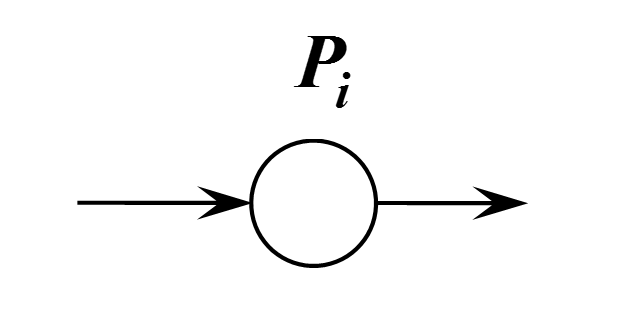
\includegraphics[width=0.7\textwidth]{place} \\ а)}
	  	\end{minipage}
	  	\hfill
	  	\begin{minipage}[ht]{0.49\linewidth}
	  		\center{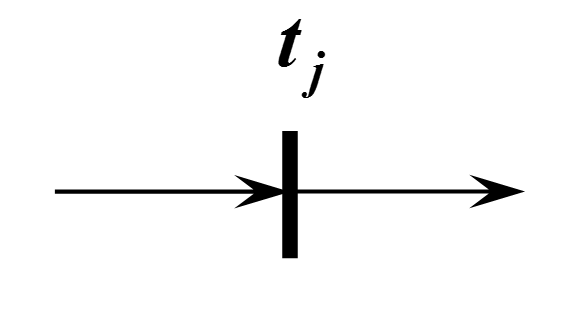
\includegraphics[width=0.8\linewidth]{tansition} \\ б)}
	  	\end{minipage}
	  	\caption{a) "--- изображение позиции, б) "--- изображение перехода. }
	  	\label{img:example}  
	  \end{figure}
	  
	  Ориентированные дуги могут соединять только позиции и переходы в прямом и обратном направлении (свойство двудольности~\cite{piterson}). Сеть Петри является мультиграфом, так как допускается кратность дуг между позициями и переходами (вершинами графа). Пример сети Петри приведен на рисунке \ref{img:petri-net}
	  
	  	\begin{figure}[h!]
	  		\center{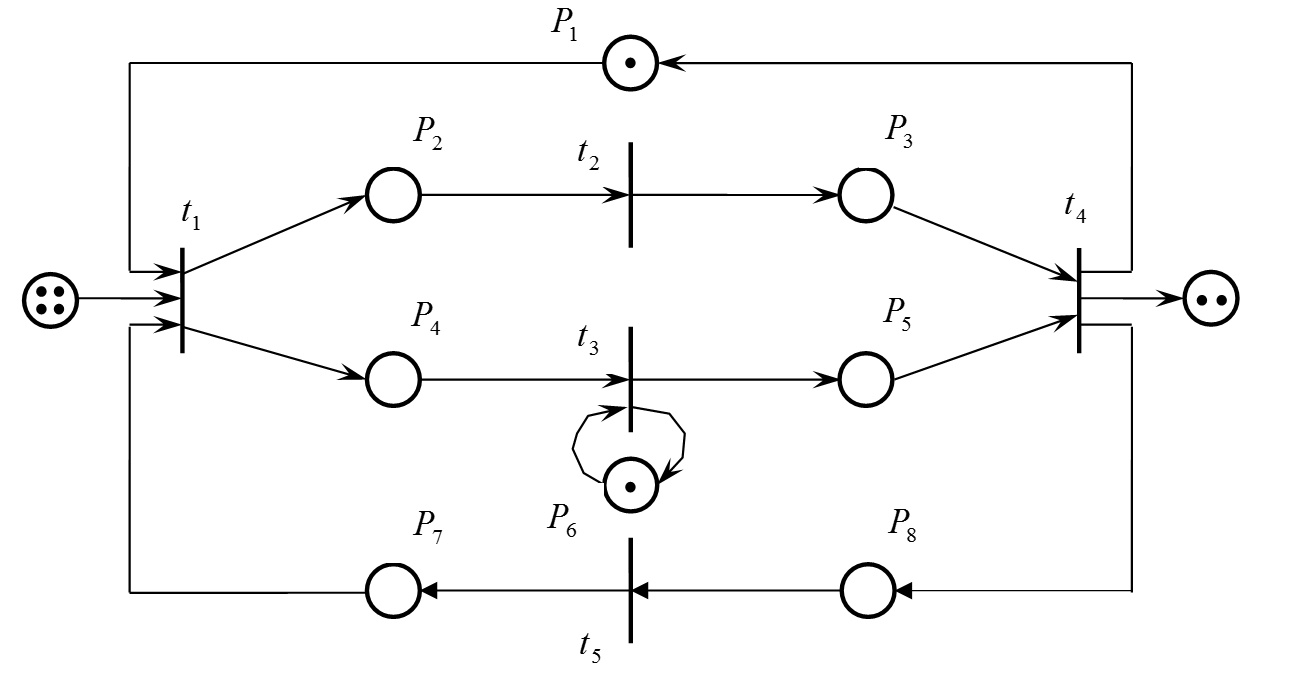
\includegraphics[width=0.7\textwidth]{petri-net}}
	  		\caption{Пример сети петри.}
	  		\label{img:petri-net}
	  	\end{figure}
	  
	  Сетью Петри принято называть тройку $<G, m_0,\rho>$  , где  $G\equiv<P,T,I,O>$ "--- граф сети Петри, $P$   "--- конечное множество позиций (или мест) сети, $T$ "--- конечное множество переходов сети, $P \cap T = \varnothing$. $I,O:T\rightarrow P^{()}$  "--- функции, задающие комплекты входных и, соответственно, выходных позиций переходов сети (здесь $P^{()}$  "--- множество всевозможных конечных комплектов элементов мно-жества $P$ ). $M \cong P^{()}$ "--- множество всевозможных состояний сети (маркировок).  $m_0 \in M$ "--- начальная маркировка сети, задающая начальное состояние сети, $\rho:T\rightarrow C$ "--- функция раскраски, возможно частичная, где $C$  "--- множество красок.
	  
	  Сеть называется ограниченной, если $ (\forall p \in P) (\exists k \in \textit{nat}) (\forall m \in \mu_0) (m(p) \leq k)$, то есть множество достижимых в сети маркировок конечно.
	  
	Ограниченная сеть Петри $S$ на множестве позиций $P$, $|P|\in \aleph_0$, может быть представлена следуюзим образом~\cite{falkTheory}:\\ 
	$ S \subseteq P^{()} \times (P^{()} \times P^{()}) $
	
	Неограниченная сеть Петри $S$ на  $P$, $|P|\in \aleph_0$:	$ S \subseteq P^{()} \times 2^{P^{()} \times P^{()}} $
	
	Для любой сети Петри $S\equiv < m_0, T >,\;  m_0 \in P^{()}$ называется начальной разметкой сети, а направленное квазиотношение $T$ -- множество переходов сети.
	
	Сети Петри рассматриваются с точностью до изоморфизма: две сети $S'\equiv<{m'}_0, T'>$ на $P'$ и $S''\equiv<{m''}_0, T''>$ на $P''$ изоморфны ($ S' \sim S'' $), если существует взаимооднозначное соответствие $ \varepsilon:P'\leftrightarrow P'' $, такое, что $ \varepsilon(T') = T'' $. Графическое представление сетей Петри хорошо известно и не нуждается в уточнении.
	
	Бинарное отношение $\mathrm{T}(T)$ изменения разметок на множестве $P^{()}$ разметок сети Петри $S\equiv < m_0, T >$:
	\begin{center}
		$\mathrm{T}(T)\cong\{<p',p''-p_1+p_2>|<p_1,p_2> \in T \wedge p_1\leq p''\}$
	\end{center}

	История поведения стандартной ограниченной сети Петри $S\equiv < m_0, T >$: кортеж $<m_0,m_1,...,m_k>$, 
	такой, что $(\forall i \in 1..k)(<m_{i-1}, m_i> \in \mathrm{T}(T))$
	
	Множество всех возможных историй поведения сети Петри $S$ обозначим $\mu(S)$.
	
	Две сети Петри $S_1$ и $S_2$ эквивалентны, если $\mu(S_1) \sim \mu(S_2)$ (т.е. существует взаимно-однозначное соответствие $\varepsilon:P'\leftrightarrow P''$, такое, что $\varepsilon(\mu(S')) = \mu(S'')$)
	
  \subsection{Сети Петри со строгой дисциплиной изменения разметок}
	Бинарное отношение $\bar{\mathrm{T}}(T)$ строгого изменения разметок на множестве $P^{()}$ 
	разметок сети в сети Петри $S\equiv < m_0, T >$~\cite{falkTheory}:
	\begin{equation}
		\begin{multlined}
			\bar{\mathrm{T}}(T)\cong\{<p',p''-p_1+p_2>|<p_1,p_2> \in T \wedge p_1\leq p'' \wedge\\
			\wedge (\exists<{p'}_1, {p''}_2> \in T)(p_1 < {p'}_1 \wedge {p'}_1 \leq p'') \}
		\end{multlined}
	\end{equation}
	  
	История поведения ограниченной сети Петри $S\equiv < m_0, T >$ со строгим изменением разметок: кортеж  $<m_0,m_1,...,m_k>$, 
	такой, что\\ $(\forall i \in 1..k)(<m_{i-1}, m_i> \in \bar{\mathrm{T}}(T))$
	  
	Пусть задана стандартная ограниченная сеть Петри $S\equiv < m_0, T >$. Пополним множество $P$ ее позиций множеством $P_G$ новых элементов,
	взаимно-однозначно соответствующих переходам из $G$: $P'\cong P\cup P_G$,\\ 
	$P_G\cong \{p_t|(t\in T)\wedge (p_t \notin P)\}$. Искомую ограниченную сеть Петри со строгой дисциплиной изменения разметок 
	обозначим $S'\equiv  < {m'}_0, T >$:\\
	${m'}_0\cong m_0 +\displaystyle\sum_{p_t\in P_G}c_{p_t}$,
	$T'\cong\{\alpha'+c_{p_{<\alpha',\alpha''>}}, \alpha'' +c_{<p_{\alpha',\alpha''>}}|<\alpha',\alpha''> \in T\} $.
	Доказательство эквивалентности сетей $S$ и $S'$ очевидно.
  \subsection{Динамические вычислительные сети}
	 % Для отображения символа в большом варианте использовать \displaystyle
	Пусть 
	$ D = \displaystyle\bigcup_{\theta\in\Theta} D_\theta $  - многосортный \textit{универсум данных},  
	где $\Theta$ - конечное множество \textit{сортов} данных, 
	$D_\theta$ - подмножество \textit{данных} сорта $\theta\in\Theta$.\\
	Будем считать, что одним из таких сортов данных является сорт \textit{nat}, такой, что $D_{\textit{nat}} \cong \aleph_0$.
	Функциональным базисом будем называть конечное множество  $ B $   всюду определенных вычислимых~\cite{falkTheory} функций вида:\\
	$ \beta: \displaystyle\bigtimes_{i'\in 1..m'}D_{\theta'_{i'}} \rightarrow \displaystyle\bigtimes_{i''\in 1..m''}D_{\theta''_{i''}} $, $ m',m'' \in \aleph_0 $  , 
	где  $ <m',m''> $   называется арностью функции $ \beta $  , а  $ <\nu',\nu''> $  , $ \nu'\in \Theta^{<m'>}, \nu''\in \Theta^{m''}  $ -- ее типом.
	\subsubsection{Определение}
		\textit{ Динамической вычислительной сетью} (\textbf{ДВС}) в функциональном базисе $B$ 
		назовем пару $<\bar{\Sigma},\dot{S}>$, где $\overline{\Sigma}$ 
		- конечное множество классов сетей ДВС, $\dot{S}$ - аксиома ДВС.
		 
		Каждый класс $\Sigma$ характеризуется: 
		уникальным именем  $\dot{\Sigma}$, 
		типом функции 
		$< |\bar{\theta}'(\dot{\Sigma})|,|\bar{\theta}''(\dot{\Sigma})|>$
		,  и конечным упорядоченным множеством $S^*(\dot{\Sigma})$
		\textit{образов сетей} этого класса.
		Тип или арность может указываться,
		при необходимости, в виде правого верхнего индекса.
		 
		Все образцы сетей из $S^*(\dot{\Sigma})$ имеют тот же тип, а, следовательно,
		и арность, что и сам класс $\Sigma$.
		Тип или арность образца сети   $S\in\bar{S}(\dot{\Sigma})$ ,
		при необходимости, также может указываться в виде его правого верхнего индекса.
		 
		Образец сети  $S\in{S^*(\dot{\Sigma})}$   в общем случае имеет вид:
		\begin{center}
			$S\cong<P,\delta,I,O,T_T,T_H,\nu',\nu'',I_T,O_T,\sigma,\rho,\varphi_T,\lambda_I,\lambda_O,\mu_0> $,где
		\end{center}
		\begin{itemize}
		  \item $P$ 
		  "--- конечное множество элементов\footnote{Используемый здесь термин «элемент сети» является, во-многом, аналогом терминов «позиция» или «место» в теории сетей Петри и «точка сети» в теории направленных отношений.}
		    образца сети,
		 
		  \item $\delta:P \rightarrow \Theta$  "--- задает сорта элементов образца сети,
		  \item  $I,O \in P^{<>}$ "--- кортежи входных и выходных элементов образца сети, \mbox{$<\delta(I),\delta(O)>$}  "---  тип, а $<|I|,|O|>$   "--- арность образца сети,
		  
		  \item $T_T$ 
		  "--- конечное множество терминальных переходов,
		  
		  \item $T_H$ 
		  "--- конечное множество нетерминальных переходов,
		    $T_T \cap T_H = \varnothing$  , $T\cong  T_T \cup T_H$ , $T \cap P = \varnothing$ ,
		 
		  \item	для всех $ t \in T$  : $I_T(t) \in P^{<\nu'(t)>}$ ,
		   $ O_T(t) \in P^{\nu''(t)} $  ;\\
		    $<\nu'(t), \nu''(t)>$   "--- \textit{арность перехода}  $ t \in T $   ( $ \nu',\nu'':T\rightarrow\aleph_0 $ ),\\
		  $ <\delta(I_T(t)),\delta(O_T(t))> $  "--- \textit{тип перехода} $t$  , 
		  
		  \item $ \sigma:T_H \rightarrow \{ \dot{\Sigma}\;| \;\Sigma \in \bar{\Sigma} \} $ (сопоставляет имена классов сетей-объектов нетерминальным переходам),
		  
		  \item $ \rho:T_H \rightarrow \Re_0 $ (задает \textit{временные сдвиги} для нетерминальных переходов),
		  
		  \item $ \omega:T_H \rightarrow P $(задает \textit{управляющие входы} нетерминальных переходов), для всех  $ t \in T_H $  $ \delta(\omega(t)) = \textit{nat} $   ;
		  
		  \item $ \varphi_T:T_T \rightarrow B $ – \textit{семантика} терминальных переходов, причем для всех  $ t \in T_T $    тип  $\varphi_T(t)$    равен  $ <\delta(I_T(t)),\delta(O_T(t))> $  ,
		  
		  \item $ \lambda_I:\{ <t,i'>|\;t\in T_T \wedge i' \in 1..\nu'(t) \} \rightarrow \Re_0 $ и
		  
		  \item $ \lambda_O:\{ <t,i''>|\;t\in T_T \wedge i'' \in 1..\nu''(t) \} \rightarrow \Re_0 $ задают «задержки» входных и выходных связей терминальных переходов с элементами образца сети,
		  
		  \item $ \mu_0 \in M_S $ , 
		  где $ M_S \cong \{ \mu\;|\; (\forall p \in P)(\mu(p) \in (D_{\delta(p)} \times \Re_0)^{()} \} $.
		  Компонент $ \mu_0 $    является, в определенном смысле, аналогом понятия маркировки сетей Петри,
		  в связи с чем множество  $ M_S $   будем тоже называть \textit{множеством возможных маркировок} сети,
		  а $\mu_0$   – ее \textit{начальной маркировкой}.
		  Не ограничивая общности, далее будем считать, что для любой маркировки  $\mu\in M_S$
		  все комплекты  $\mu(p)$  (для всех $p \in P$ ) представлены кортежами вида 
		  $ < <d_1,\tau_1>,...,<d_{|\mu(p)|}, \tau_{|\mu(p)|} > $  , 
		  построенными из элементов соответствующего комплекта так, 
		  что компоненты кортежей упорядочены по неубыванию вторых компонентов пар 
		  (т.е. $ (\forall i\in 1..|\mu|-1) (\tau_i \leq \tau_{i+1}) $~). 
		\end{itemize}
		 
		 \newtheorem{com}{Замечание}
		 \begin{com}\label{izomorph}
		 		Заметим, что образцы сетей рассматриваются с точностью до $(P, T_T, T_H)$-изоморфизма.
		 \end{com}
		 
		\textit{ Аксиома} или, по-иному, инициальное состояние $\dot{S}$ ДВС (корень дерева состояний) -- один из образцов некоторого класса $\Sigma \in \bar{\Sigma}$.
	\subsubsection{Графическое представление ДВС}
		Графическое представление ДВС опишем как совокупность графических представлений множества $\bar{\Sigma}$ классов 
		и сети $\dot{S}$ - аксиомы ДВС (рисунок \ref{img:DNC-graphic})
		\begin{figure}[h!]
			\center{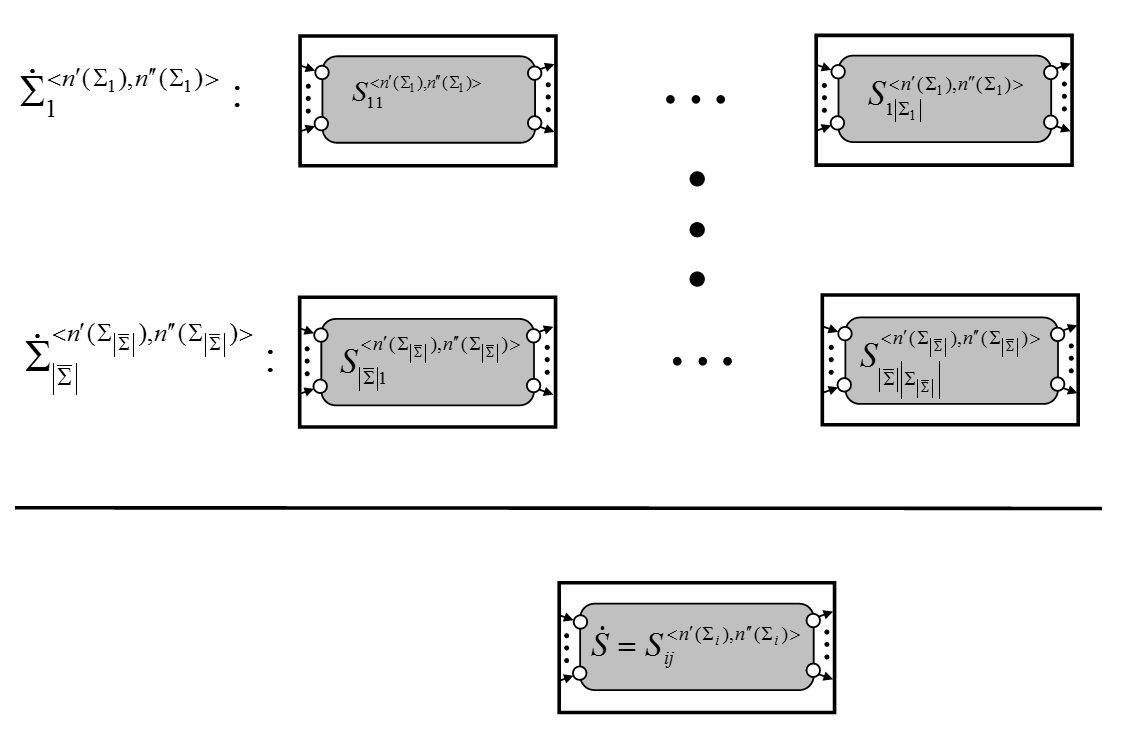
\includegraphics[width=0.8\textwidth]{DNC-graphic}}
			\caption{Графическое представление ДВС.}
			\label{img:DNC-graphic}
		\end{figure}
		
		\begin{figure}[h!]
			\begin{minipage}[ht]{0.49\linewidth}
				\center{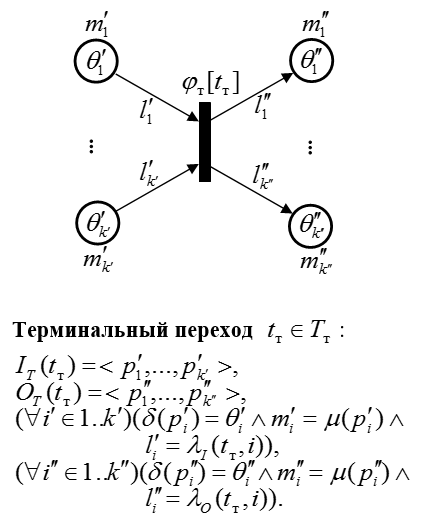
\includegraphics[width=0.8\linewidth]{terminal-t} \\ а)}
			\end{minipage}
			\hfill
			\begin{minipage}[ht]{0.49\linewidth}
				\center{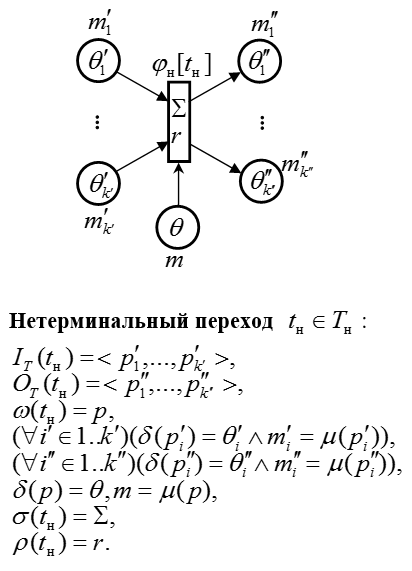
\includegraphics[width=0.8\linewidth]{non-terminal-t} \\ б)}
			\end{minipage}
			\caption{Графическое представление компонентов сетей.}
			\label{img:components}  
		\end{figure}
		
		Графическое представление класса $\Sigma$ включает имя $\dot{\Sigma}$ этого класса 
		и множество графических представлений образцов сетей этого класса. За основу представления сетей (образцов сетей) 
		взято представление сетей отношений в теории направленных отношений, представление элементов сети и переходов 
		фактически заимствовано из наиболее часто используемых представлений позиций и переходов сетей Петри 
		и их различных расширений и модификаций, а прочие компоненты в графическом представлении указываются 
		в качестве меток элементов графических представлений рассмотренных выше компонентов на рисунке \ref{img:components}.
		представлены представления терминальных и нетерминальных переходов, включая связанные с ними входные и выходные элементы сети.
		%Рис 4. %TODO вставить ссылку на рисунок
		%содержит пример представления ДВС.

	
	\subsubsection{Процесс в ДВС}
		\textit{Процесс} в ДВС -- прадерево смены состояний ДВС (далее -- дерево состояний). Дерево состояний строится на основе определения готовности к срабатыванию терминальных и нетерминальных переходов и определения нового состояния ДВС в результате срабатывания некоторого перехода из числа готовых к срабатыванию согласно правилу выбора перехода.
		За основу этого правила принята описанная выше строгая дисциплина срабатывания переходов, уточнение которой приведено ниже. Если согласно этой дисциплине возможно срабатывание нескольких переходов, то срабатывание каждого из них определяет свою ветвь в дереве состояний.
	
	\paragraph{Правило выбора переходов}

		Пусть $ S\cong<P,\delta,I,O,T_T,T_H,\nu',\nu'',I_T,O_T,\sigma,\rho,\varphi_T,\lambda_I, \lambda_O,\mu> $
		-- текущее состояние ДВС.  Готовность к срабатыванию переходов в любые моменты времени определяется значением
		предиката $ U:T\times\Re_0\rightarrow\{true,false\} $.
		
		Для определения значения $ U(t,\tau) $    для терминальных переходов $t\in T_T$
		введем вспомогательный предикат  $ {U^{i,l}_T} $     
		с двумя параметрами $ i\in \aleph_0 $   и $ l:P\rightarrow\aleph_0 $  .
		Для  $ t\in T_T $   положим $ U(t,\tau)\cong {U^{1,l_0}}_T(t,\tau) $  ,
		где $ (\forall p\in P)(l_0(p) = 0) $  , и $ I_T(t)=<{p_1}',...,{p_{\nu'(t)}}' > $   .
		Тогда 
		\begin{equation}
			{U^{i,l}}_T(t,\tau)\cong
			\begin{cases}
				true, \quad \text{если}\; i > \nu'(t),\\
				U^{i+1,l'}_T(t,\tau)\wedge(l(p_i')\leq|\mu(p_i')|)\wedge(\mu(p_i')(l(p_i')) (2) +\lambda_I(t,i)\leq \tau),\\
				\quad \text{где } l'(p_i')=l(p_i')+1, (\forall p \not= p_i')(l'(p_i')=l(p_i'), \quad \text{если } i\leq \nu'(t)
			\end{cases}
		\end{equation}
		
		Если   $ t\in T_H $ , то	
		\begin{equation}
			U(t,\tau)\cong(|\mu(\omega(t))|>0)\wedge(head(\mu(\omega(t)))(2)\leq \tau).
		\end{equation}
		
		Переход  $ t\in T $   может сработать в момент времени  $ \tau\in\Re_0 $   и образовать свою ветвь в дереве состояний,
		если он готов к срабатыванию и нет готовых к срабатыванию в тот же момент времени более приоритетных переходов.
		Используемая строгая дисциплина срабатывания переходов предполагает, 
		что переход $ t\in T $ имеет более высокий приоритет, чем переход  $ t'\in T $  ,
		если $ (\forall\mu \in M_S)(\forall \tau \in \Re_0) (U(t,\tau)\supset U(t',\tau) $  .
		
		Наконец, определим новое состояние ДВС, находившейся в состоянии $ S $  , 
		после срабатывания в момент времени   $ \tau \in \Re_0 $  некоторого перехода. 
		Отдельно рассмотрим случай  $ t\in T_T $   и случай  $ t\in T_H $ . 
		Обозначим новое состояние в результате срабатывания этого перехода как  $ \vec{S} $ . 
		Пусть $ \tau $   -- минимально возможное время, в которое может сработать какой-то переход $ t\in T $  .
		\begin{enumerate}
			\item Если  $ t\in T_T $ , то
			$ \vec{S}\cong<P,\delta,I,O,T_T,T_H,\nu',\nu'',I_T,O_T,\sigma,\rho,\varphi_T,\lambda_I,\lambda_O,\vec{\mu} >$, 
			где новая маркировка $ \vec{\mu} $  определяется выполнением следующего алгоритма, использующего, 
			помимо параметра цикла $ i:\aleph_0$\footnote{Запись $x:\chi$ означает, что программная переменная $x$ имеет область значений $\chi$}   и вспомогательной переменной $ p:P $  , 
			две «переменные»  $ arg:\displaystyle\bigtimes_{i'\in 1..\nu'(t)}D_{\delta(p_{i'}')} $, 
			$ val: \displaystyle\bigtimes_{i''\in 1..\nu''(t)} D_{\delta(p_{i''}'')} $  
			для хранения, соответственно, значения аргумента и значения функции $ \varphi_T $  , представляющей семантику терминального перехода:\\
			
			\begin{minipage}[ht]{0.8\textwidth}
	\begin{algorithm}[H]
		\Begin
		{
			$\bar{\mu}:=\mu$;\\
			$i:=1 $;\\
			$ arg:=<> $;\\
			\While{$ i\leq \nu'(t) $}
			{
				$ p:=I_T(t)(i) $;\\
				$ arg:=arg<head(\vec{\mu}(p))(1)> $;\\
				$ \vec{\mu}(p):=tail(\mu(p)) $;\\
				$ i:=i+1 $;\\	
			}
			$ val:=\phi_T(t)(arg) $;\\
			$ i:=1 $;\\
			\While{$ val\not=<> $}
			{
				$ p:=O_T(t)(i) $;\\
				$ \vec{\mu}(p):=\vec{\mu}(p)+1_{<head(val),\tau+\lambda_O(<t,O_T(t)(i)>) } $;\\
				$ val:=tail(val) $
			}
		}
		
		\caption{Алгоритм нахождения маркировки.}
	\end{algorithm}
\end{minipage}

			\item Если $ t\in T_H $  , $ p=\omega(t) $ , то сеть $ \vec{S} $    
			будет получена подстановкой сдвинутого во времени образца сети  $ S^*(\sigma(t))[head(\mu(p))(1)] $   
			(с начальной маркировкой  $ \bar{\mu}_0 $ ) в сеть $ S $    вместо нетерминального перехода $ t $ , 
			с предварительным удалением «головного» элемента из кортежа $ \mu(p) $: $ \mu(p):=tail(\mu(p)) $ .
		\end{enumerate}
	\paragraph{Срабатывание перехода}		
		Пусть  $ \bar{S}\equiv<\bar{P},\bar{\delta},\bar{I},\bar{O},
		\bar{T}_T,\bar{T}_H,\bar{\nu}',\bar{\nu}'',\bar{I}_T,\bar{O}_T,\bar{\sigma},
		\bar{\rho},\bar{\varphi}_T,\bar{\lambda}_I,\bar{\lambda}_O,\bar{\mu}> $ , где все компоненты $ \bar{S} $   , кроме $ \bar{\mu} $  ,
		взяты из упомянутого образца сети, а сдвиг во времени означает, что для всех  $ p\in \bar{P} $ ,  
		если \( \bar{\mu}_0(p)=<<d_1,\tau_1>,...,<d_k,\tau_k>>\) , то $ \bar{\mu}(p)=<<d_1,\tau_1+(\tau+\rho(t))>,...,<d_k,\tau_k+(\tau+\rho(t))>> $  , 
		т.е. вторые компоненты элементов начальной маркировки в подставляемом образце интерпретируются как временные интервалы 
		относительно момента времени его срабатывания, сдвинутые дополнительно индивидуально для конкретного нетерминального перехода. 
		
		Результат  $ \vec{S} $    подстановки сети   $ \bar{S} $   в сеть   $ S $  вместо ее нетерминального перехода  $ t\in T_H $   
		определяется во многом аналогично тому, как определена операция подстановки для сетевых представлений направленных отношений.
		
		Согласно \textit{Замечанию~\ref{izomorph}} будем считать, что 
		$ P\cap\bar{P} = \emptyset $, 
		$ T_T\cap\bar{T}_T=\emptyset $, 
		$ T_H\cap \bar{T}_H=\emptyset $.
		Определим отношение эквивалентности, обозначаемое инфиксом $ \approx $ , как рефлексивное, симметричное, транзитивное замыкание бинарного отношения 
		$ \{ <I_T(t)(i),\bar{I}(i)>|i\in 1..\nu'(t) \} \cup \{<O_T(t)(i),\bar{O}(i)>|i \in 1..\nu''(t) \} $. 
		Множество элементов полученной в результате подстановки сети определим как фактор множества  $ P\cap\bar{P} $  по отношению  $ \approx : \vec{P}\cong(P\cup\bar{P})\;/\approx$, 
		а для определения всех остальных компонентов  $ \vec{S} $  (функции рассматриваются как графики) произведем в покомпонентном объединении сетей  $ S $   и $ \bar{S} $   
		замену элементов из $ P\cup\bar{P} $ на соответствующие элементы из  $ \vec{P} $  (на классы эквивалентности, в которые они входят):\\
		\begin{equation}
		\begin{multlined}
		\vec{S}\cong[(\forall p \in P \cup \bar{P} )(p\Rightarrow(p\; / \approx) )] 
		<P\cup\bar{P},\delta\cup\bar{\delta},I\cup\bar{I},O\cup\bar{O},T_T\cup\bar{T}_T,\\
		T_H\cup\bar{T}_H,\nu'\cup\bar{\nu}',\nu''\cup\bar{\nu}'',I_T\cup\bar{I}_T,
		O_T\cup\bar{O}_T,\sigma\cup\bar{\sigma},\rho\cup\bar{\rho},\varphi_T\cup\bar{\varphi}_T,
		\lambda_I\cup\bar{\lambda}_I,\\
		\lambda_O\cup\bar{\lambda}_O,\mu\cup\bar{\mu}>
		\end{multlined}
		\end{equation}
		
		Для выполнения операции замены в объединении графиков функций, 
		область определения которых пересекается с областью  $ P\cup\bar{P} $  объектов замены, требуется уточнение. 
		Для случая $ [(\forall p \in P \cup \bar{P} )(p\Rightarrow(p\; / \approx) )](\delta\cup\bar{\delta})$   
		проблем не возникает, и можно воспользоваться общим правилом:\\
		$[(\forall p \in P \cup \bar{P} )(p\Rightarrow(p\; / \approx) )](\delta\cup\bar{\delta}) \cong
		[(\forall p \in P \cup \bar{P} )(p\Rightarrow(p\; / \approx) )] \delta \cup [(\forall p \in P \cup \bar{P} )(p\Rightarrow(p\; / \approx) )]\bar{\delta}$,\\
		так как в результате объединения результатов замены получится функциональный график, 
		а для случая  $ [(\forall p \in P \cup \bar{P} )(p\Rightarrow(p\; / \approx) )](\mu\cup\bar{\mu}) $   
		в результате объединения результатов замены график может оказаться не функциональным. 
		Поэтому для случая, когда замена осуществляется в графике функции с областью определения  $ P\cup\bar{P} $  
		и значениями-комплектами из множеств  $ (D_{\delta(p)}\times\Re_0) $  для всех $ p\in P\cup \bar{P} $, 
		результат замены определим по иному:\\
		$ [(\forall p \in P \cup \bar{P} )(p\Rightarrow(p\; / \approx) )](\mu\cup\bar{\mu})\cong
		\{<p',\!\displaystyle\sum_{p \in (p'/\approx)}\!(\mu\cup\bar{\mu})(p)| p' \in ((P\cup\bar{P}) /\!\approx) \} $.
		
   \subsubsection{Сборка <<мусора>>  в ДВС}
	   Мусором в состояниях-вершинах дерева состояний ДВС мы будем называть 
	   \begin{enumerate}
		   \item переходы состояния, которые заведомо не смогут сработать ни в одном из подчиненных состояний, т.е. в других состояниях, к которым из этого состояния есть путь в дереве состояний,
		   \item элементы состояний, используемые во всех подчиненных состояниях исключительно как входные и выходные элементы исключаемых «мусорных» переходов.
	   \end{enumerate}

	   Мусор исключается из всех подчиненных состояний того состояния в дереве, в котором для перехода или для элемента установлен статус «мусора».
	   
	   Алгоритм выявления мусора во многом подобен алгоритму сборки мусора при выполнении программ в большинстве реализаций языков программирования. Он предполагает выполнение следующих шагов:
	   \begin{enumerate}
		   \item первоначально все переходы и элементы сети полагаются мусорными;
		   \item отмечаем как немусорные переходы, все входные элементы которых имеют непустую маркировку (в том числе и переходы с пустым кортежем входных позиций),  либо отмечены как немусорные;
		   \item отмечаем как немусорные элементы, являющиеся выходными для не-мусорных переходов;
		   \item повторяем шаги 2 и 3 до тех пор, пока при их выполнении отмечается как немусорный хотя бы еще один новый переход или элемент.
	   \end{enumerate}
	   
	   Оставшиеся переходы, не отмеченные как немусорные, удаляются из сети, вместе с элементами ассоциированных с ними графиков функций. %Оставшиеся элементы, не отмеченные как немусорные, ...